\documentclass[11pt]{article}
\pagestyle{plain}
\usepackage{latexsym,exscale,amsfonts,amsmath,amssymb,array}
\usepackage{color}
\usepackage[colorlinks]{hyperref}
\setlength{\topmargin}{-2.3cm}
\setlength{\textheight}{23.8cm}
\setlength{\oddsidemargin}{-0.5cm}
\setlength{\textwidth}{17cm}
\setlength{\parindent}{0cm}
\setlength{\parskip}{.4cm}
\newcommand{\totaldiffx}{\frac{d}{dx}}
\newcommand{\pardiffx}{\frac{\partial}{\partial x}}
\newcommand{\luft}{\:\!}

\usepackage{graphicx}
\usepackage[latin1]{inputenc}
\usepackage{mathpazo}
\usepackage[T1]{fontenc}
\usepackage[comma,numbers,sort&compress]{natbib}


\begin{document}
\begin{center}
\large \bf Computational Astrophysics \rm \\
2019\\
{\small Exercises 06. Root Finding}
\end{center}

\begin{enumerate}

\item {\bf Eccentric Anomaly}
\begin{center}
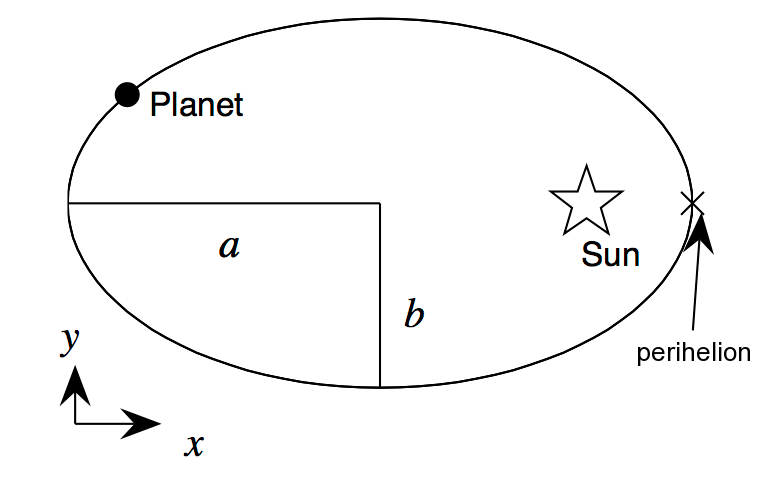
\includegraphics[width=0.55\textwidth]{orbit.png}
\vspace*{-0.5cm}
\end{center}

A planet is moving around the sun in an elliptic Keplerian orbit with
semi-major axis $a$, semi-minor axis $b$, and eccentricity $e =
\sqrt{1 - b^2/a^2}$.  The planet last perihelion occur at $t=0$.  The angular frequency of the motion is $\omega = 2\pi / T$, where $T$ is the duration of its orbit (period).

If we define a 2D coordinate system $(x,y)$ with origin at the center
of the ellipse, then the points on the ellipse are described by the
equation
\begin{equation}
\frac{x^2}{a^2} + \frac{y^2}{b^2} = 1\,\,.
\end{equation}
The location of the planet in the $(x,y)$ coordinate system is given
by 
\begin{equation}
\begin{aligned}
x &= a \cos E\,\,,\\
y &= b \sin E\,\,,
\end{aligned}
\end{equation}
where $E$ is the \emph{eccentric anomaly}, which is defined by
\begin{equation}
E = \omega t + e \sin E\,\,.
\label{eq:int}
\end{equation}


The interesting equation here is Eq.~(\ref{eq:int}), which gives an \emph{implicit}
non-linear relationship for E. In order to find $E$ for a given $\omega t$ and
$e$, we will need to find the solution to the following equation:
\begin{equation}
0 = E - \omega t - e \sin E\,\,,
\end{equation}
in other words, we have to find this equation's root!


\begin{enumerate}
\item[(a)] The Earth has an orbital period of $365.25635\,\text{days}$,
a semi-major axis $a = 1.496\times 10^8\,\mathrm{km} = 1\,\mathrm{AU}$,
and its orbit has an eccentricity of $e = 0.0167$. Compute $E$, $x$ and $y$
for $t = 91\,\text{days}$, $t = 182\,\text{days}$, and $t = 273\,\text{days}$
using your favorite root finding method. The fractional error in $E$ at the end
of your computation (from one iteration to the next) should be less than
$10^{-10}$. How many iterations does your method need, i.e, how quickly does it
converge?

\item[(b)] Now suppose that something (very bad) happened,
  putting Earth on a pretty eccentric orbit, say $e = 0.99999$. How
  many iterations does your algorithm need now? How could you
  accelerate convergence?
\end{enumerate}

\item {\bf Polynomials with Multiple Roots}

Find all real roots of
\begin{equation}
f(x) = 3x^5 + 5x^4 - x^3\,\,.
\end{equation}
How many are there and how can you construct an algorithm that finds
all of them? This method should be general and should work for real
roots of any polynomial in one variable with at least on real
root. You may ask the internet for help!

Implement your method and be ready to be tested in class to demonstrate its capabilities
with a few examples.
\end{enumerate}

Happy Coding :) !

\end{document}
